%# -*- coding:utf-8 -*-
\documentclass[10pt,aspectratio=43,mathserif]{beamer}		
%设置为 Beamer 文档类型,设置字体为 10pt,长宽比为4:3,数学字体为 serif 风格

%%%%-----导入宏包-----%%%%
\usepackage{ccnu}			%导入 CCNU 模板宏包
\usepackage{xeCJK}			%导入 ctex 宏包,添加中文支持
\usepackage{amsmath,amsfonts,amssymb,bm}   %导入数学公式所需宏包
\usepackage{color}			 %字体颜色支持
\usepackage{graphicx,hyperref,url}
\usepackage{metalogo}	% 非必须
\usepackage{fontspec}
\usepackage{bibentry}
\usepackage{graphicx} % Allows including images
\usepackage{booktabs} % Allows the use of \toprule, \midrule and \bottomrule in tables
\usepackage{url}
%% 上文引用的包可按实际情况自行增删
%%%%%%%%%%%%%%%%%%	


\beamertemplateballitem		%设置 Beamer 主题

%%%%------------------------%%%%%
\catcode`\。=\active         %或者=13
\newcommand{。}{.}				
%将正文中的“。”号转换为“.”。中文标点国家规范建议科技文献中的句号用圆点替代
%%%%%%%%%%%%%%%%%%%%%

%%%%----首页信息设置----%%%%
\title[Research on High School Math Exercise Recommendation Based on Graph Neural Network]{Research on High School Math Exercise Recommendation Based on Graph Neural Network}
%\subtitle{——这里是副标题}			
%%%%----标题设置


\author[Wangzhihui Mei]{
  Wangzhihui Mei \\\medskip
  Supervisor: Zhifeng Wang%
  }
%%%%----个人信息设置
  
\institute[CCNU-UOW JI]{
  Central China Normal University Wollongong Joint Institute}
%%%%----机构信息

\date[\today]{
  \today}
%%%%----日期信息
  
\begin{document}

\begin{frame}
	\titlepage
\end{frame}				%生成标题页

\section{Outline}
\begin{frame}
	\frametitle{Outline}
	\tableofcontents
\end{frame}				%生成提纲页
%------------------------------------------------
\section{Introduction}
%------------------------------------------------
\subsection{Research Background}
\subsubsection{Objectives}
\begin{frame}
	\frametitle{Research Background}
	\framesubtitle{Objectives}
	\begin{itemize}
		\item Knowledge State Monitoring
		\item Learning Resource Recommendation
		\item High School Math (Chinese)
	\end{itemize}
\end{frame}

%------------------------------------------------
\subsubsection{Existing Problems}
\begin{frame}
	\frametitle{Research Background}
	\framesubtitle{Existing Problems}
	\begin{description}
		\item[Inappropriate Recommendation] Exercise recommendation is not based on knowledge mastery
		\item[Disorganized exercise] Labelling knowledge for exercises lacking knowledge tags
		\item[Knowledge evaluation] The difficulty for obtaining knowledge mastery proficiency of the student
		\item[Exercise recommendation] How to recommend appropriate exercises according to their knowledge status
	\end{description}
\end{frame}
%------------------------------------------------
\subsection{Research Cores}
\begin{frame}
	\frametitle{Research Cores}
	\begin{block}{Exercise knowledge labeling}
		A multi-knowledge point labeling algorithm for high school mathematics exercises based on bidirectional LSTM (Bi-LSTM)~\cite{chen2017improving} and graph convolutional neural network (GCN)~\cite{kipf2016semi}.
	\end{block}
	\begin{block}{Knowledge tracing}
		An improved graph-based DKVMN~\cite{zhang2017dynamic} knowledge tracing model to evaluate the knowledge proficiency of students.
	\end{block}
	\begin{block}{Exercise recommendation}
		A mathematical exercise recommendation model based on Matching-Ranking~\cite{segev2009context}.
	\end{block}
\end{frame}
%------------------------------------------------
\section{Model and Algorithm Detail}
%------------------------------------------------
\subsection{Exercise Knowledge Labelling}
\begin{frame}
	\frametitle{Exercise Knowledge Labelling}
	\framesubtitle{Architecture}
	\begin{figure}
		\centering
		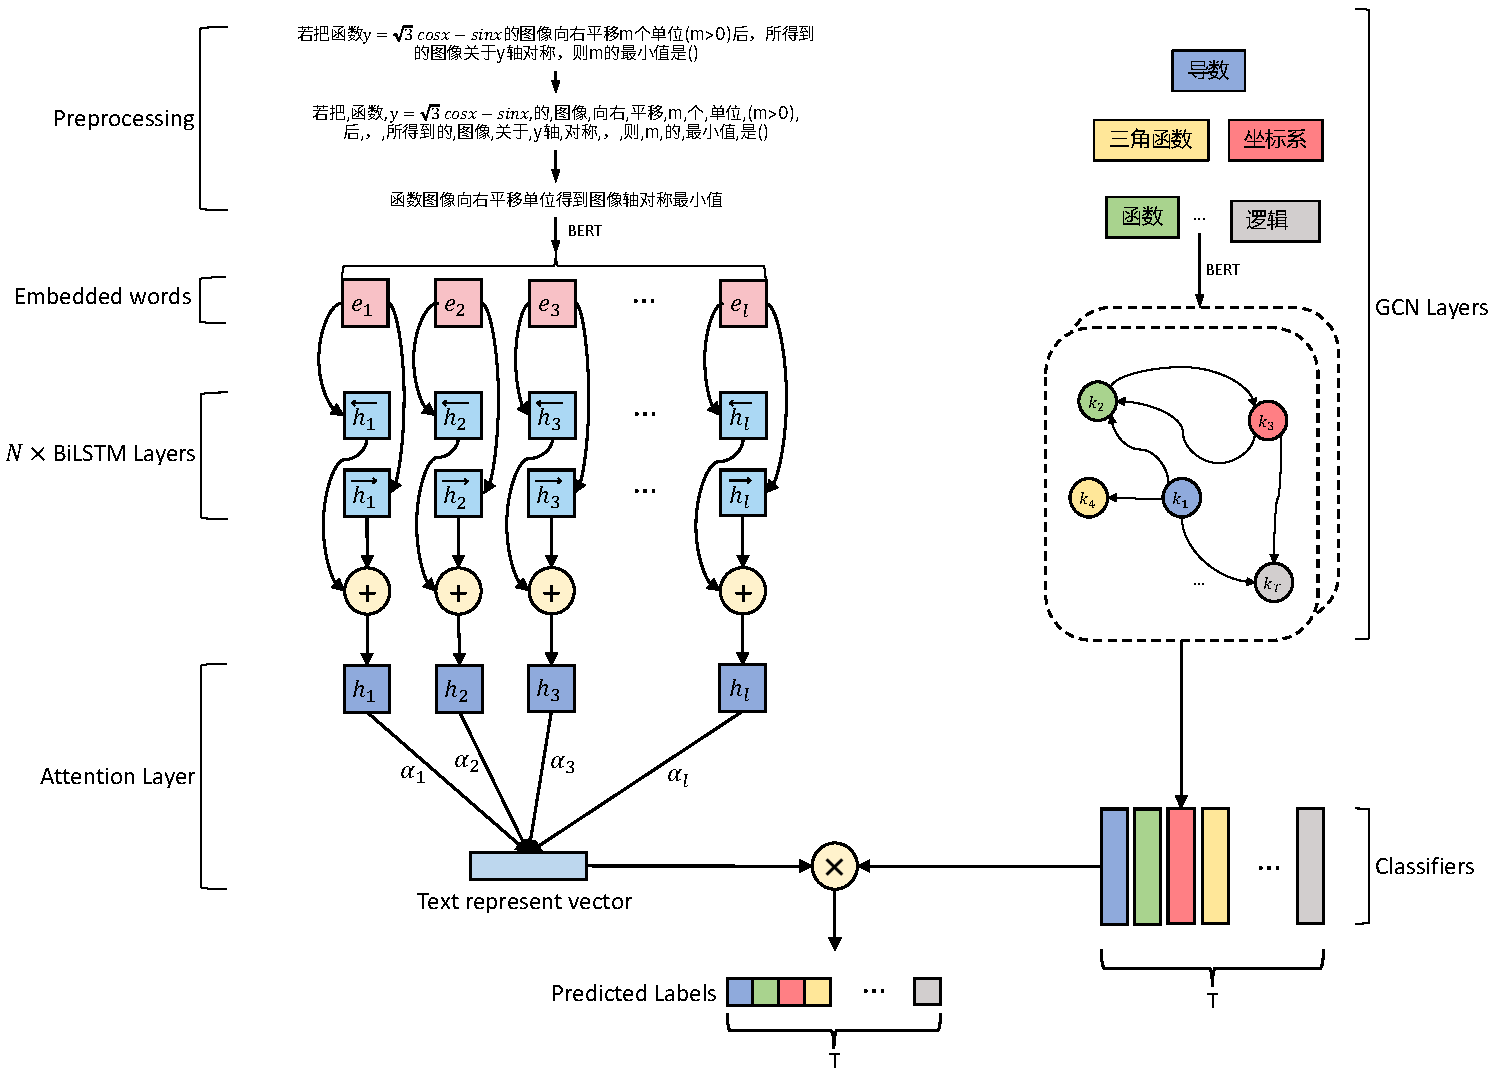
\includegraphics[height=0.80\textheight]{figures/ch2-ov.pdf}
		%\caption{Model architecture}\label{fig:ch2-archi}
	\end{figure}
\end{frame}

\begin{frame}
	\frametitle{Exercise Knowledge Labelling}
	\framesubtitle{GCN-based Classifier Generator}
	\begin{figure}
		\centering
		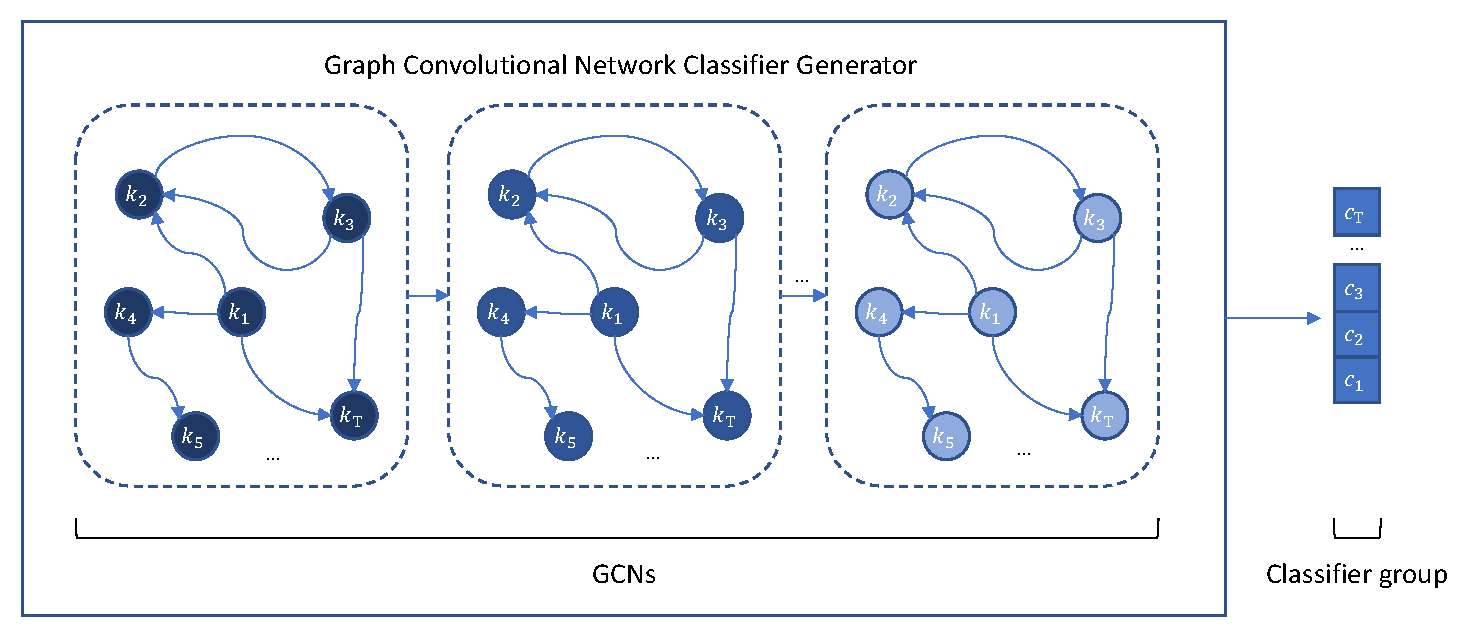
\includegraphics[width=1.0\textwidth]{figures/ch2-gcnclsgen-model.pdf}
		%\caption{Model architecture}\label{fig:ch2-archi}
	\end{figure}
\end{frame}

%------------------------------------------------
\subsection{Knowledge Tracing}

\begin{frame}
	\frametitle{Knowledge Tracing}
	\framesubtitle{Problem Description}
	\begin{figure}
		\centering
		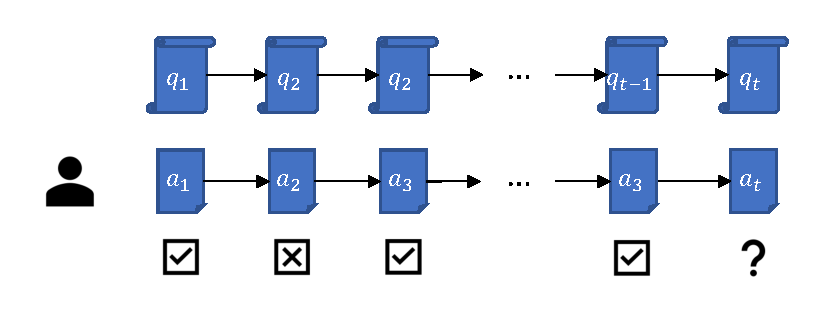
\includegraphics[width=1.0\textwidth]{figures/ch3-model-ktdes.pdf}
		\caption{Knowledge tracing modeling}
	\end{figure}
\end{frame}


\begin{frame}
	\frametitle{Knowledge Tracing}
	\framesubtitle{Architecture}
	\begin{figure}
		\centering
		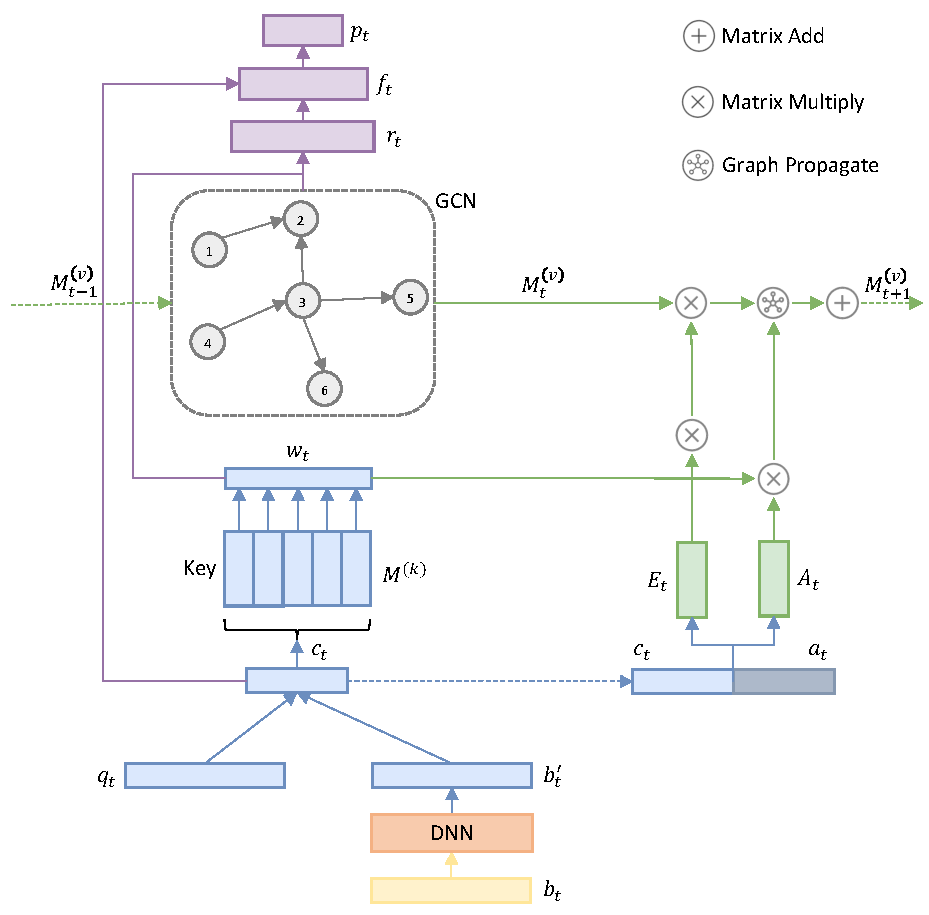
\includegraphics[height=0.80\textheight]{figures/ch3-ov.pdf}
		%\caption{The architecture of proposed knowledge tracing model}
	\end{figure}
\end{frame}




\begin{frame}
	\frametitle{Knowledge Tracing}
	\framesubtitle{Question-Knowledge Relation Modelling}
	\begin{figure}
		\centering
		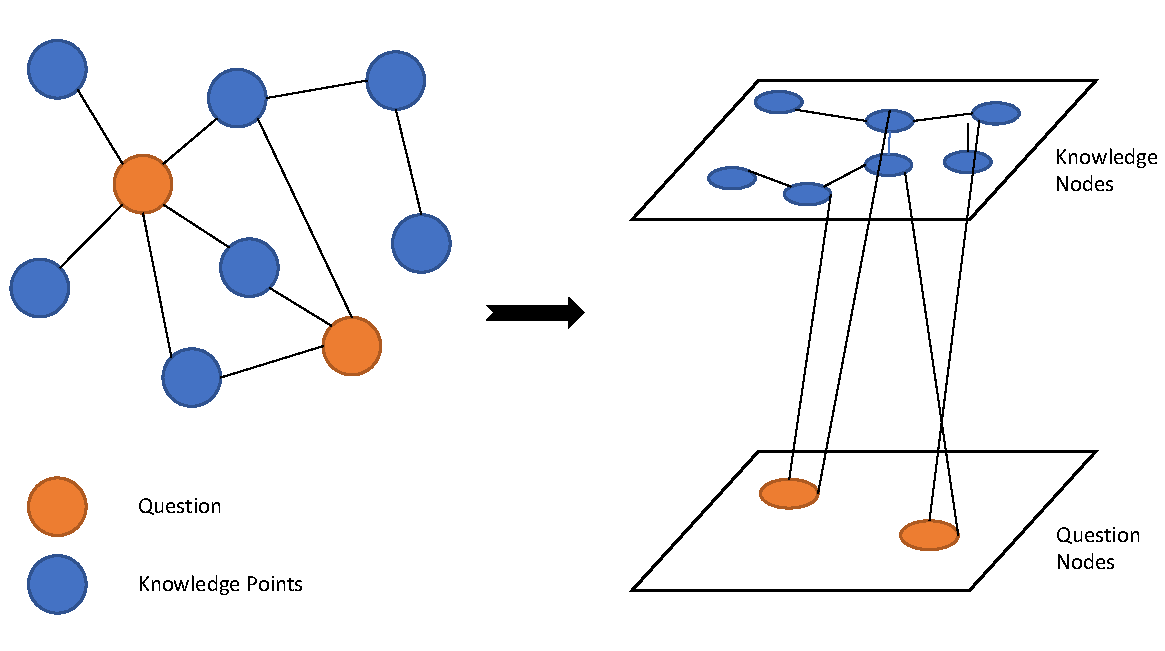
\includegraphics[width=0.94\textwidth]{figures/ch3-gat-kq.pdf}
		\caption{Relation modeling of exercise question and knowledge points}
	\end{figure}
\end{frame}




% \begin{frame}
%   \frametitle{Knowledge Tracing}
%   \framesubtitle{Detail}

% \end{frame}


\subsection{Exercise Recommendation}
\begin{frame}
	\frametitle{Exercise Recommendation}
	\framesubtitle{Architecture}
	\begin{figure}
		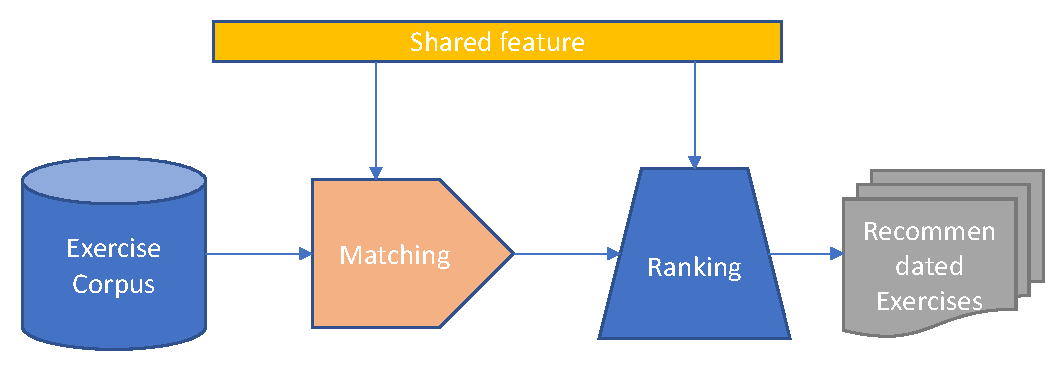
\includegraphics[width=0.9\textwidth]{figures/ch4-ov.pdf}
		\caption{The architecture of recommendation model}
	\end{figure}
\end{frame}

\begin{frame}
	\frametitle{Exercise Recommendation}
	\framesubtitle{Matching Phase}
	\begin{figure}
		\centering
		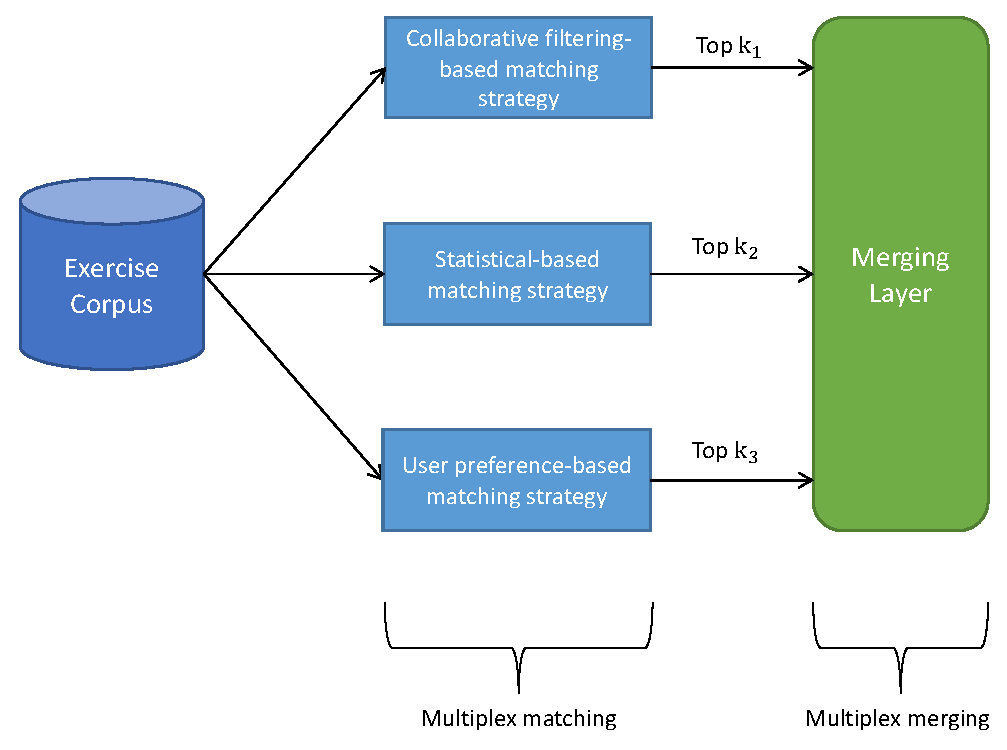
\includegraphics[height=0.7\textheight]{figures/ch4-matching-model.pdf}
		%\caption{The matching phase}
	\end{figure}
\end{frame}

\begin{frame}
	\frametitle{Exercise Recommendation}
	\framesubtitle{Ranking Phase}
	\begin{figure}
		\centering
		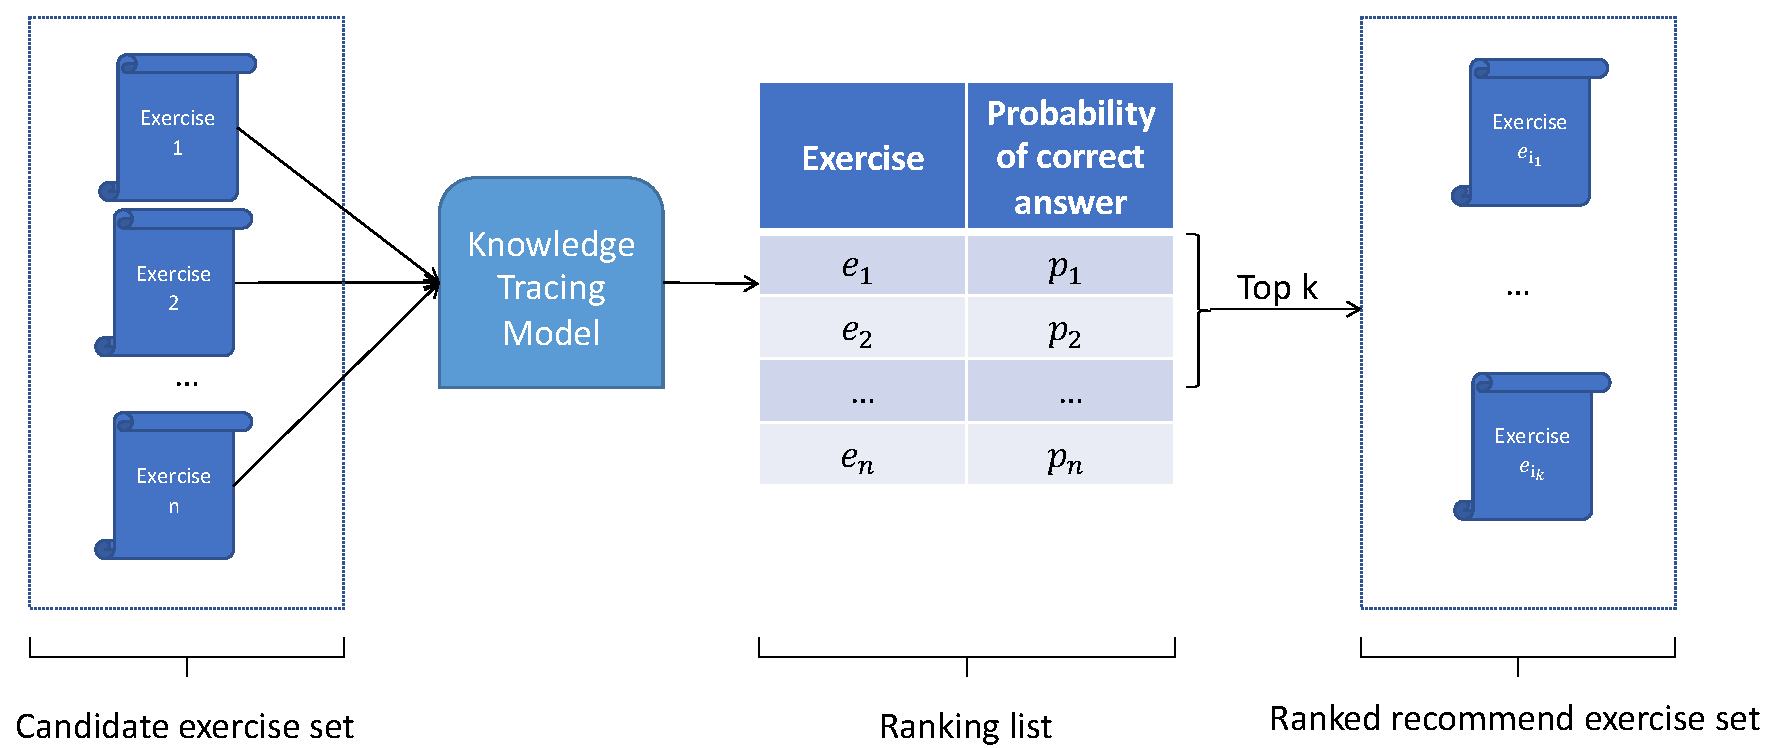
\includegraphics[width=1.0\textwidth]{figures/ch4-ranking-model.pdf}
		%\caption{The ranking phase}
	\end{figure}
\end{frame}

%------------------------------------------------
\section{Experiment and Result Analysis}
\subsection{Exercise Knowledge Labelling}
\begin{frame}
	\frametitle{Experiment Design}
	\framesubtitle{Exercise Knowledge Labelling}
	\begin{itemize}
		\item Compare with several baseline models
		\item Evaluate the multi-label classification performance
	\end{itemize}
\end{frame}

\begin{frame}
	\frametitle{Result Analysis}
	\framesubtitle{Exercise Knowledge Labeling}
	\begin{table}[htbp!]
		\caption{The performance comparison between baseline and proposed knowledge labelling models.}\label{tbl:ch2-result-bsline1}
		\centering
		\begin{tabular}{ccccc}
			\toprule
			Metrics           & \(\operatorname{F1}_{macro}\) & \(\operatorname{F1}_{micro}\) & \(\operatorname{Acc}_{ML}\) & \(\operatorname{F1}_{ML}\) \\
			\midrule
			BiLSTM+Attention  & 0.824                         & 0.924                         & 0.874                       & 0.926                      \\
			fastText          & 0.846                         & 0.922                         & 0.854                       & 0.916                      \\
			TextCNN           & 0.761                         & 0.923                         & 0.857                       & 0.917                      \\
			\textbf{Proposed} & \textbf{0.912}                & \textbf{0.932}                & \textbf{0.888}              & \textbf{0.937}             \\
			\bottomrule
		\end{tabular}
	\end{table}
\end{frame}



\begin{frame}
	\frametitle{Result Analysis}
	\framesubtitle{Exercise Knowledge Labeling}
	\begin{table}[htbp!]
		\caption{The multi-label classification performance of proposed model.}\label{tbl:ch2-result-detail}
		\centering
		\begin{tabular}{ccccc}
			\toprule
			Class          & Precision & Recall & F1 Score & Support \\
			\midrule
			三角函数       & 0.957     & 0.710  & 0.815    & 31      \\
			函数奇偶性     & 0.946     & 0.930  & 0.938    & 187     \\
			导数           & 0.918     & 0.866  & 0.892    & 247     \\
			平面向量       & 0.942     & 0.961  & 0.951    & 204     \\
			数列           & 0.996     & 0.971  & 0.983    & 243     \\
			逻辑与命题关系 & 0.958     & 0.883  & 0.919    & 180     \\
			集合           & 0.907     & 0.867  & 0.886    & 45      \\
			\midrule
			Micro avg      & 0.951     & 0.915  & 0.932    & 1137    \\
			Macro avg      & 0.946     & 0.884  & 0.912    & 1137    \\
			Weighted avg   & 0.951     & 0.915  & 0.932    & 1137    \\
			Samples avg    & 0.951     & 0.935  & 0.937    & 1137    \\
			\bottomrule
		\end{tabular}
	\end{table}
\end{frame}

\subsection{Knowledge Tracing}
\begin{frame}
	\frametitle{Experiment Design}
	\framesubtitle{Knowledge Tracing}
	\begin{block}{Basic Method}
		Compare with other KT baseline models BKT~\cite{yudelson2013individualized}, DKT~\cite{piech2015deep}, DKVMN~\cite{chen2017improving} and GKT~\cite{nakagawa2019graph}
	\end{block}
	\begin{table}[htbp!]
		\centering
		\caption{Dataset Statistics}\label{tbl:ch2-tb1}
		\scalebox{0.7}{
			\begin{tabular}{ccccc}
				\toprule
				Dataset   & \#students & \#exercises & \#knowledge points & \#interactions \\
				\midrule
				ASSIST15  & 19,917     & 102,396     & 100                & 709K           \\
				ASSIST17  & 1,709      & 4,117       & 102                & 943K           \\
				STATICS11 & 333        & 1,223       & 156                & 189K           \\
				\bottomrule
			\end{tabular}}
	\end{table}
\end{frame}


\begin{frame}
	\frametitle{Result Analysis}
	\framesubtitle{Knowledge Tracing}
	\begin{table}[htb]
		\centering
		\caption{The performance comparison between baseline and proposed knowledge tracing models.}\label{tbl:ch3-performance}
		\begin{tabular}{cccc}
			\toprule
			Model    & ACC (\%)                    & AUC (\%)                   & Training time (sec) \\
			\midrule
			DKT      & \(76.99\pm 0.08 \)          & \(81.79\pm 0.09\)          & \(2,731\)           \\
			DKVMN    & \(75.63\pm 0.19 \)          & \(79.58\pm 0.27\)          & \(3,378\)           \\
			NPA      & \(77.09\pm 0.08\)           & \(81.81\pm 0.13\)          & \(3,872\)           \\
			SAKT     & \(76.37\pm 0.15\)           & \(80.77\pm 0.09\)          & \(4,367\)           \\
			\midrule
			Proposed & \(\mathbf{81.34\pm 0.25} \) & \(\mathbf{83.20\pm 0.25}\) & \(4,597\)           \\
			\bottomrule
		\end{tabular}
	\end{table}
\end{frame}


\subsection{Exercise Recommendation}
\begin{frame}
	\frametitle{Experiment Design}
	\framesubtitle{Exercise Recommendation}
	\begin{itemize}
		\item Compared with conventional Collaborative Filtering and Random Recommendation
		\item Using adapted KT dataset for testing
		\item Check if the selected exercise is in the final recommendation list
	\end{itemize}
\end{frame}


\begin{frame}
	\frametitle{Result Analysis}
	\framesubtitle{Exercise Recommendation}
	\begin{table}[htb]
		\caption{The performance comparison between baseline and proposed recommendation models.}\label{tbl:ch4-exp-result}
		\centering
		\setlength{\tabcolsep}{7mm}{
			\begin{tabular}{cc c }
				\toprule
				Model    & ACC             & AUC             \\
				\midrule
				CF       & 0.6329          & 0.6627          \\
				DKT      & 0.7741          & 0.7906          \\
				\midrule
				Proposed & \textbf{0.7997} & \textbf{0.7923} \\
				\bottomrule
			\end{tabular}}
	\end{table}
\end{frame}


\section{Conclusion}
\begin{frame}
	\frametitle{Conclusion}
	\begin{itemize}
		\item The three modules of the proposed model satisfy the requirements of the design
		\item The proposed model achieves better performance compared with baseline models.
	\end{itemize}
\end{frame}
%------------------------------------------------

\begin{frame}[allowframebreaks]{References}
	\bibliographystyle{plain}
	%\bibliographystyle{amsalpha}
	%\bibliography{mybeamer} also works
	\bibliography{./ref.bib}
\end{frame}

%------------------------------------------------

\begin{frame}
	\Huge{\centerline{The End}}
\end{frame}
\end{document}